% Options for packages loaded elsewhere
\PassOptionsToPackage{unicode}{hyperref}
\PassOptionsToPackage{hyphens}{url}
\PassOptionsToPackage{dvipsnames,svgnames,x11names}{xcolor}
%
\documentclass[
  letterpaper,
  DIV=11,
  numbers=noendperiod]{scrartcl}

\usepackage{amsmath,amssymb}
\usepackage{lmodern}
\usepackage{iftex}
\ifPDFTeX
  \usepackage[T1]{fontenc}
  \usepackage[utf8]{inputenc}
  \usepackage{textcomp} % provide euro and other symbols
\else % if luatex or xetex
  \usepackage{unicode-math}
  \defaultfontfeatures{Scale=MatchLowercase}
  \defaultfontfeatures[\rmfamily]{Ligatures=TeX,Scale=1}
\fi
% Use upquote if available, for straight quotes in verbatim environments
\IfFileExists{upquote.sty}{\usepackage{upquote}}{}
\IfFileExists{microtype.sty}{% use microtype if available
  \usepackage[]{microtype}
  \UseMicrotypeSet[protrusion]{basicmath} % disable protrusion for tt fonts
}{}
\makeatletter
\@ifundefined{KOMAClassName}{% if non-KOMA class
  \IfFileExists{parskip.sty}{%
    \usepackage{parskip}
  }{% else
    \setlength{\parindent}{0pt}
    \setlength{\parskip}{6pt plus 2pt minus 1pt}}
}{% if KOMA class
  \KOMAoptions{parskip=half}}
\makeatother
\usepackage{xcolor}
\setlength{\emergencystretch}{3em} % prevent overfull lines
\setcounter{secnumdepth}{-\maxdimen} % remove section numbering
% Make \paragraph and \subparagraph free-standing
\ifx\paragraph\undefined\else
  \let\oldparagraph\paragraph
  \renewcommand{\paragraph}[1]{\oldparagraph{#1}\mbox{}}
\fi
\ifx\subparagraph\undefined\else
  \let\oldsubparagraph\subparagraph
  \renewcommand{\subparagraph}[1]{\oldsubparagraph{#1}\mbox{}}
\fi

\usepackage{color}
\usepackage{fancyvrb}
\newcommand{\VerbBar}{|}
\newcommand{\VERB}{\Verb[commandchars=\\\{\}]}
\DefineVerbatimEnvironment{Highlighting}{Verbatim}{commandchars=\\\{\}}
% Add ',fontsize=\small' for more characters per line
\usepackage{framed}
\definecolor{shadecolor}{RGB}{241,243,245}
\newenvironment{Shaded}{\begin{snugshade}}{\end{snugshade}}
\newcommand{\AlertTok}[1]{\textcolor[rgb]{0.68,0.00,0.00}{#1}}
\newcommand{\AnnotationTok}[1]{\textcolor[rgb]{0.37,0.37,0.37}{#1}}
\newcommand{\AttributeTok}[1]{\textcolor[rgb]{0.40,0.45,0.13}{#1}}
\newcommand{\BaseNTok}[1]{\textcolor[rgb]{0.68,0.00,0.00}{#1}}
\newcommand{\BuiltInTok}[1]{\textcolor[rgb]{0.00,0.23,0.31}{#1}}
\newcommand{\CharTok}[1]{\textcolor[rgb]{0.13,0.47,0.30}{#1}}
\newcommand{\CommentTok}[1]{\textcolor[rgb]{0.37,0.37,0.37}{#1}}
\newcommand{\CommentVarTok}[1]{\textcolor[rgb]{0.37,0.37,0.37}{\textit{#1}}}
\newcommand{\ConstantTok}[1]{\textcolor[rgb]{0.56,0.35,0.01}{#1}}
\newcommand{\ControlFlowTok}[1]{\textcolor[rgb]{0.00,0.23,0.31}{#1}}
\newcommand{\DataTypeTok}[1]{\textcolor[rgb]{0.68,0.00,0.00}{#1}}
\newcommand{\DecValTok}[1]{\textcolor[rgb]{0.68,0.00,0.00}{#1}}
\newcommand{\DocumentationTok}[1]{\textcolor[rgb]{0.37,0.37,0.37}{\textit{#1}}}
\newcommand{\ErrorTok}[1]{\textcolor[rgb]{0.68,0.00,0.00}{#1}}
\newcommand{\ExtensionTok}[1]{\textcolor[rgb]{0.00,0.23,0.31}{#1}}
\newcommand{\FloatTok}[1]{\textcolor[rgb]{0.68,0.00,0.00}{#1}}
\newcommand{\FunctionTok}[1]{\textcolor[rgb]{0.28,0.35,0.67}{#1}}
\newcommand{\ImportTok}[1]{\textcolor[rgb]{0.00,0.46,0.62}{#1}}
\newcommand{\InformationTok}[1]{\textcolor[rgb]{0.37,0.37,0.37}{#1}}
\newcommand{\KeywordTok}[1]{\textcolor[rgb]{0.00,0.23,0.31}{#1}}
\newcommand{\NormalTok}[1]{\textcolor[rgb]{0.00,0.23,0.31}{#1}}
\newcommand{\OperatorTok}[1]{\textcolor[rgb]{0.37,0.37,0.37}{#1}}
\newcommand{\OtherTok}[1]{\textcolor[rgb]{0.00,0.23,0.31}{#1}}
\newcommand{\PreprocessorTok}[1]{\textcolor[rgb]{0.68,0.00,0.00}{#1}}
\newcommand{\RegionMarkerTok}[1]{\textcolor[rgb]{0.00,0.23,0.31}{#1}}
\newcommand{\SpecialCharTok}[1]{\textcolor[rgb]{0.37,0.37,0.37}{#1}}
\newcommand{\SpecialStringTok}[1]{\textcolor[rgb]{0.13,0.47,0.30}{#1}}
\newcommand{\StringTok}[1]{\textcolor[rgb]{0.13,0.47,0.30}{#1}}
\newcommand{\VariableTok}[1]{\textcolor[rgb]{0.07,0.07,0.07}{#1}}
\newcommand{\VerbatimStringTok}[1]{\textcolor[rgb]{0.13,0.47,0.30}{#1}}
\newcommand{\WarningTok}[1]{\textcolor[rgb]{0.37,0.37,0.37}{\textit{#1}}}

\providecommand{\tightlist}{%
  \setlength{\itemsep}{0pt}\setlength{\parskip}{0pt}}\usepackage{longtable,booktabs,array}
\usepackage{calc} % for calculating minipage widths
% Correct order of tables after \paragraph or \subparagraph
\usepackage{etoolbox}
\makeatletter
\patchcmd\longtable{\par}{\if@noskipsec\mbox{}\fi\par}{}{}
\makeatother
% Allow footnotes in longtable head/foot
\IfFileExists{footnotehyper.sty}{\usepackage{footnotehyper}}{\usepackage{footnote}}
\makesavenoteenv{longtable}
\usepackage{graphicx}
\makeatletter
\def\maxwidth{\ifdim\Gin@nat@width>\linewidth\linewidth\else\Gin@nat@width\fi}
\def\maxheight{\ifdim\Gin@nat@height>\textheight\textheight\else\Gin@nat@height\fi}
\makeatother
% Scale images if necessary, so that they will not overflow the page
% margins by default, and it is still possible to overwrite the defaults
% using explicit options in \includegraphics[width, height, ...]{}
\setkeys{Gin}{width=\maxwidth,height=\maxheight,keepaspectratio}
% Set default figure placement to htbp
\makeatletter
\def\fps@figure{htbp}
\makeatother

\KOMAoption{captions}{tableheading}
\makeatletter
\makeatother
\makeatletter
\makeatother
\makeatletter
\@ifpackageloaded{caption}{}{\usepackage{caption}}
\AtBeginDocument{%
\ifdefined\contentsname
  \renewcommand*\contentsname{Table of contents}
\else
  \newcommand\contentsname{Table of contents}
\fi
\ifdefined\listfigurename
  \renewcommand*\listfigurename{List of Figures}
\else
  \newcommand\listfigurename{List of Figures}
\fi
\ifdefined\listtablename
  \renewcommand*\listtablename{List of Tables}
\else
  \newcommand\listtablename{List of Tables}
\fi
\ifdefined\figurename
  \renewcommand*\figurename{Figure}
\else
  \newcommand\figurename{Figure}
\fi
\ifdefined\tablename
  \renewcommand*\tablename{Table}
\else
  \newcommand\tablename{Table}
\fi
}
\@ifpackageloaded{float}{}{\usepackage{float}}
\floatstyle{ruled}
\@ifundefined{c@chapter}{\newfloat{codelisting}{h}{lop}}{\newfloat{codelisting}{h}{lop}[chapter]}
\floatname{codelisting}{Listing}
\newcommand*\listoflistings{\listof{codelisting}{List of Listings}}
\makeatother
\makeatletter
\@ifpackageloaded{caption}{}{\usepackage{caption}}
\@ifpackageloaded{subcaption}{}{\usepackage{subcaption}}
\makeatother
\makeatletter
\@ifpackageloaded{tcolorbox}{}{\usepackage[many]{tcolorbox}}
\makeatother
\makeatletter
\@ifundefined{shadecolor}{\definecolor{shadecolor}{rgb}{.97, .97, .97}}
\makeatother
\makeatletter
\makeatother
\ifLuaTeX
  \usepackage{selnolig}  % disable illegal ligatures
\fi
\IfFileExists{bookmark.sty}{\usepackage{bookmark}}{\usepackage{hyperref}}
\IfFileExists{xurl.sty}{\usepackage{xurl}}{} % add URL line breaks if available
\urlstyle{same} % disable monospaced font for URLs
\hypersetup{
  pdftitle={Predicting Fire Suppression Calls},
  pdfauthor={Angela Zhao},
  colorlinks=true,
  linkcolor={blue},
  filecolor={Maroon},
  citecolor={Blue},
  urlcolor={Blue},
  pdfcreator={LaTeX via pandoc}}

\title{Predicting Fire Suppression Calls}
\author{Angela Zhao}
\date{9/30/24}

\begin{document}
\maketitle
\ifdefined\Shaded\renewenvironment{Shaded}{\begin{tcolorbox}[enhanced, sharp corners, interior hidden, breakable, frame hidden, borderline west={3pt}{0pt}{shadecolor}, boxrule=0pt]}{\end{tcolorbox}}\fi

\hypertarget{introduction}{%
\section{Introduction}\label{introduction}}

Accurately predicting fire suppression calls can significantly enhance
emergency response planning and resource allocation. This analysis aims
to develop a predictive model to forecast the timing of fire suppression
calls using historical data. We will employ techniques such as
Bootstrap, Principal Component Analysis (PCA), and Neural Networks with
backpropagation to achieve this goal.

\hypertarget{data-preparation}{%
\section{Data Preparation}\label{data-preparation}}

We begin by loading the necessary libraries and importing the dataset.
The data comes from the Baltimore County firehouse and includes data
starting from 2015. Importantly, we extract the hour of the call from
the time column of the Excel.

\begin{Shaded}
\begin{Highlighting}[]
\CommentTok{\# Load libraries}
\FunctionTok{library}\NormalTok{(tidyverse)}
\FunctionTok{library}\NormalTok{(lubridate)}
\FunctionTok{library}\NormalTok{(rsample)}
\FunctionTok{library}\NormalTok{(hms)}
\FunctionTok{library}\NormalTok{(timeDate)}
\FunctionTok{library}\NormalTok{(ggplot2)}
\FunctionTok{library}\NormalTok{(openxlsx)}
\FunctionTok{library}\NormalTok{(here)}
\FunctionTok{library}\NormalTok{(viridis)}
\FunctionTok{library}\NormalTok{(ggpubr)}
\end{Highlighting}
\end{Shaded}

\begin{Shaded}
\begin{Highlighting}[]
\CommentTok{\# Load data}
\NormalTok{data }\OtherTok{\textless{}{-}} \FunctionTok{read.xlsx}\NormalTok{(}\FunctionTok{here}\NormalTok{(}\StringTok{"data"}\NormalTok{, }\StringTok{"raw"}\NormalTok{, }\StringTok{"Call stats.xlsx"}\NormalTok{), }
                  \AttributeTok{sheet =} \StringTok{"Supression Only"}\NormalTok{) }\SpecialCharTok{\%\textgreater{}\%} 
  \FunctionTok{mutate}\NormalTok{(}\AttributeTok{time =}\NormalTok{ time }\SpecialCharTok{*} \DecValTok{86400}\NormalTok{, }
         \AttributeTok{dispatched =} \FunctionTok{as.Date}\NormalTok{(dispatched, }\AttributeTok{origin =} \StringTok{"1899{-}12{-}30"}\NormalTok{)) }

\CommentTok{\# Reformat call time and dispatch date to datetime object}
\NormalTok{data }\OtherTok{\textless{}{-}}\NormalTok{ data }\SpecialCharTok{\%\textgreater{}\%}
  \FunctionTok{mutate}\NormalTok{(}\AttributeTok{time\_formatted =}\NormalTok{ hms}\SpecialCharTok{::}\FunctionTok{as\_hms}\NormalTok{(time))}

\NormalTok{data }\OtherTok{\textless{}{-}}\NormalTok{ data }\SpecialCharTok{\%\textgreater{}\%}
  \FunctionTok{mutate}\NormalTok{(}\AttributeTok{datetime =} \FunctionTok{as.POSIXct}\NormalTok{(}\FunctionTok{paste}\NormalTok{(dispatched, time\_formatted), }\AttributeTok{format =} \StringTok{"\%Y{-}\%m{-}\%d \%H:\%M:\%S"}\NormalTok{))}

\NormalTok{data}\SpecialCharTok{$}\NormalTok{block }\OtherTok{=} \FunctionTok{as.factor}\NormalTok{(data}\SpecialCharTok{$}\NormalTok{block) }\SpecialCharTok{\%\textgreater{}\%} \FunctionTok{ordered}\NormalTok{(}\AttributeTok{levels =}\FunctionTok{c}\NormalTok{(}\StringTok{"12 AM {-} 2 AM"}\NormalTok{, }
                                                         \StringTok{"2 AM {-} 4 AM"}\NormalTok{, }
                                                         \StringTok{"4 AM {-} 6 AM"}\NormalTok{, }
                                                         \StringTok{"6 AM {-} 8 AM"}\NormalTok{,}
                                                         \StringTok{"8 AM {-} 10 AM"}\NormalTok{,}
                                                         \StringTok{"10 AM {-} 12 PM"}\NormalTok{,}
                                                         \StringTok{"12 PM {-} 2 PM"}\NormalTok{,}
                                                          \StringTok{"2 PM {-} 4 PM"}\NormalTok{, }
                                                         \StringTok{"4 PM {-} 6 PM"}\NormalTok{, }
                                                         \StringTok{"6 PM {-} 8 PM"}\NormalTok{,}
                                                         \StringTok{"8 PM {-} 10 PM"}\NormalTok{,}
                                                         \StringTok{"10 PM {-} 12 AM"}\NormalTok{))}

\CommentTok{\# Extract additional time{-}based features}
\NormalTok{data }\OtherTok{\textless{}{-}}\NormalTok{ data }\SpecialCharTok{\%\textgreater{}\%}
  \FunctionTok{mutate}\NormalTok{(}\AttributeTok{hour =} \FunctionTok{hour}\NormalTok{(datetime),}
         \AttributeTok{day =} \FunctionTok{day}\NormalTok{(datetime),}
         \AttributeTok{month =} \FunctionTok{month}\NormalTok{(datetime),}
         \AttributeTok{year =} \FunctionTok{year}\NormalTok{(datetime))}
\end{Highlighting}
\end{Shaded}

\hypertarget{data-exploration}{%
\subsection{Data Exploration}\label{data-exploration}}

In this brief exploratory analysis, we see that there are not large
distinctions across months of the year or across days of the week.
Likewise, there are not large distinctions in the number of calls
between holidays v.s. non-holidays and weekends v.s. weekdays.

\begin{Shaded}
\begin{Highlighting}[]
\CommentTok{\# Plot calls by day of week}
\NormalTok{p\_day }\OtherTok{=}\NormalTok{ data }\SpecialCharTok{\%\textgreater{}\%}
  \FunctionTok{count}\NormalTok{(Day.of.week) }\SpecialCharTok{\%\textgreater{}\%}
  \FunctionTok{ggplot}\NormalTok{(}\FunctionTok{aes}\NormalTok{(}\AttributeTok{x =} \FunctionTok{reorder}\NormalTok{(Day.of.week, n), }\AttributeTok{y =}\NormalTok{ n)) }\SpecialCharTok{+}
  \FunctionTok{geom\_bar}\NormalTok{(}\AttributeTok{stat =} \StringTok{"identity"}\NormalTok{, }\AttributeTok{fill =} \StringTok{"steelblue"}\NormalTok{) }\SpecialCharTok{+}
  \FunctionTok{labs}\NormalTok{(}\AttributeTok{title =} \StringTok{"Number of Calls by Day of Week"}\NormalTok{, }
       \AttributeTok{x =} \StringTok{"Day of Week"}\NormalTok{, }\AttributeTok{y =} \StringTok{"Number of Calls"}\NormalTok{) }\SpecialCharTok{+}
  \FunctionTok{coord\_flip}\NormalTok{() }\SpecialCharTok{+} \FunctionTok{theme\_minimal}\NormalTok{()}

\FunctionTok{ggsave}\NormalTok{(p\_day, }\AttributeTok{filename =} \FunctionTok{here}\NormalTok{(}\StringTok{"docs"}\NormalTok{, }\StringTok{"figures"}\NormalTok{, }\StringTok{"hist\_dayofweek.png"}\NormalTok{))}

\CommentTok{\# Plot calls by month}
\NormalTok{p\_month }\OtherTok{=}\NormalTok{ data }\SpecialCharTok{\%\textgreater{}\%}
  \FunctionTok{count}\NormalTok{(month) }\SpecialCharTok{\%\textgreater{}\%}
  \FunctionTok{ggplot}\NormalTok{(}\FunctionTok{aes}\NormalTok{(}\AttributeTok{x =} \FunctionTok{reorder}\NormalTok{(}\FunctionTok{factor}\NormalTok{(month, }\AttributeTok{labels =} \FunctionTok{c}\NormalTok{(}\StringTok{"January"}\NormalTok{, }\StringTok{"February"}\NormalTok{, }\StringTok{"March"}\NormalTok{,}
                                          \StringTok{"April"}\NormalTok{, }\StringTok{"May"}\NormalTok{, }\StringTok{"June"}\NormalTok{, }\StringTok{"July"}\NormalTok{, }\StringTok{"August"}\NormalTok{,}
                                          \StringTok{"September"}\NormalTok{, }\StringTok{"October"}\NormalTok{, }\StringTok{"November"}\NormalTok{, }
                                          \StringTok{"December"}\NormalTok{)),n), }\AttributeTok{y =}\NormalTok{ n)) }\SpecialCharTok{+}
  \FunctionTok{geom\_bar}\NormalTok{(}\AttributeTok{stat =} \StringTok{"identity"}\NormalTok{, }\AttributeTok{fill =} \StringTok{"lightblue"}\NormalTok{) }\SpecialCharTok{+}
  \FunctionTok{labs}\NormalTok{(}\AttributeTok{title =} \StringTok{"Number of Calls by Month"}\NormalTok{, }
       \AttributeTok{x =} \StringTok{"Month"}\NormalTok{, }\AttributeTok{y =} \StringTok{"Number of Calls"}\NormalTok{) }\SpecialCharTok{+}
  \FunctionTok{coord\_flip}\NormalTok{() }\SpecialCharTok{+} \FunctionTok{theme\_minimal}\NormalTok{()}
\FunctionTok{ggsave}\NormalTok{(p\_month, }\AttributeTok{filename =} \FunctionTok{here}\NormalTok{(}\StringTok{"docs"}\NormalTok{, }\StringTok{"figures"}\NormalTok{, }\StringTok{"hist\_month.png"}\NormalTok{))}

\CommentTok{\# Create heat map of day of week v.s. hour}
\CommentTok{\# Aggregate calls by day\_of\_week and block}
\NormalTok{aggregated\_data }\OtherTok{\textless{}{-}}\NormalTok{ data }\SpecialCharTok{\%\textgreater{}\%}
  \FunctionTok{group\_by}\NormalTok{(Day.of.week, block) }\SpecialCharTok{\%\textgreater{}\%}
  \FunctionTok{summarise}\NormalTok{(}\AttributeTok{call\_count =} \FunctionTok{n}\NormalTok{()) }\SpecialCharTok{\%\textgreater{}\%}
  \FunctionTok{ungroup}\NormalTok{()}

\CommentTok{\# Ensure the day\_of\_week is ordered from Monday to Sunday}
\NormalTok{aggregated\_data}\SpecialCharTok{$}\NormalTok{day\_of\_week }\OtherTok{\textless{}{-}} \FunctionTok{factor}\NormalTok{(aggregated\_data}\SpecialCharTok{$}\NormalTok{Day.of.week, }
                                     \AttributeTok{levels =} \FunctionTok{c}\NormalTok{(}\StringTok{"Monday"}\NormalTok{, }\StringTok{"Tuesday"}\NormalTok{, }\StringTok{"Wednesday"}\NormalTok{, }\StringTok{"Thursday"}\NormalTok{, }
                                                \StringTok{"Friday"}\NormalTok{, }\StringTok{"Saturday"}\NormalTok{, }\StringTok{"Sunday"}\NormalTok{))}

\CommentTok{\# Create the heatmap}
\NormalTok{p\_heatmap }\OtherTok{\textless{}{-}} \FunctionTok{ggplot}\NormalTok{(aggregated\_data, }\FunctionTok{aes}\NormalTok{(}\AttributeTok{x =}\NormalTok{ block, }\AttributeTok{y =}\NormalTok{ day\_of\_week, }\AttributeTok{fill =}\NormalTok{ call\_count)) }\SpecialCharTok{+}
  \FunctionTok{geom\_tile}\NormalTok{(}\AttributeTok{color =} \StringTok{"white"}\NormalTok{, }\AttributeTok{width =} \FloatTok{0.9}\NormalTok{, }\AttributeTok{height =} \FloatTok{0.9}\NormalTok{) }\SpecialCharTok{+}  \CommentTok{\# Adjust width here}
  \FunctionTok{scale\_fill\_viridis}\NormalTok{(}\AttributeTok{name =} \StringTok{"Number of Calls"}\NormalTok{, }\AttributeTok{option =} \StringTok{"G"}\NormalTok{) }\SpecialCharTok{+}
  \FunctionTok{labs}\NormalTok{(}
    \AttributeTok{title =} \StringTok{"Heatmap of Fire Suppression Calls by Time of Day and Day of Week"}\NormalTok{,}
    \AttributeTok{x =} \StringTok{"Time Block"}\NormalTok{,}
    \AttributeTok{y =} \StringTok{"Day of Week"}
\NormalTok{  ) }\SpecialCharTok{+}
  \FunctionTok{theme\_minimal}\NormalTok{() }\SpecialCharTok{+}
  \FunctionTok{theme}\NormalTok{(}
    \AttributeTok{axis.text.x =} \FunctionTok{element\_text}\NormalTok{(}\AttributeTok{angle =} \DecValTok{90}\NormalTok{, }\AttributeTok{hjust =} \DecValTok{1}\NormalTok{),}
    \AttributeTok{panel.grid =} \FunctionTok{element\_blank}\NormalTok{()}
\NormalTok{  ) }\SpecialCharTok{+}
  \FunctionTok{coord\_fixed}\NormalTok{(}\AttributeTok{ratio =} \FloatTok{0.5}\NormalTok{)}

\FunctionTok{ggsave}\NormalTok{(p\_heatmap, }\AttributeTok{filename =} \FunctionTok{here}\NormalTok{(}\StringTok{"docs"}\NormalTok{, }\StringTok{"figures"}\NormalTok{, }\StringTok{"heatmap.png"}\NormalTok{))}

\CommentTok{\#ggarrange(p\_day, p\_month, p\_heatmap)}
\end{Highlighting}
\end{Shaded}

\begin{figure}

\begin{minipage}[t]{0.50\linewidth}

{\centering 

\raisebox{-\height}{

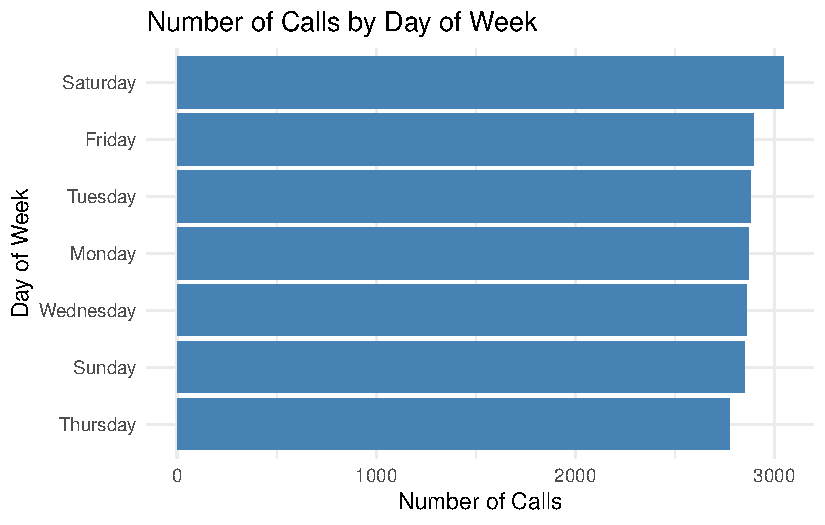
\includegraphics{Report_files/figure-pdf/exploratory_1-1.pdf}

}

\caption{Calls per Day of Week}

}

\end{minipage}%
%
\begin{minipage}[t]{0.50\linewidth}

{\centering 

\raisebox{-\height}{

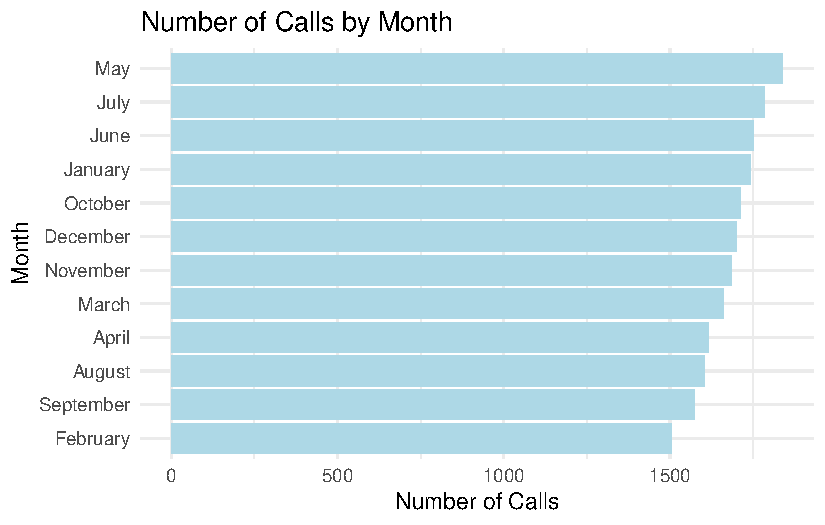
\includegraphics{Report_files/figure-pdf/exploratory_1-2.pdf}

}

\caption{Calls per Month}

}

\end{minipage}%

\end{figure}

\begin{figure}

\begin{minipage}[t]{\linewidth}

{\centering 

\raisebox{-\height}{

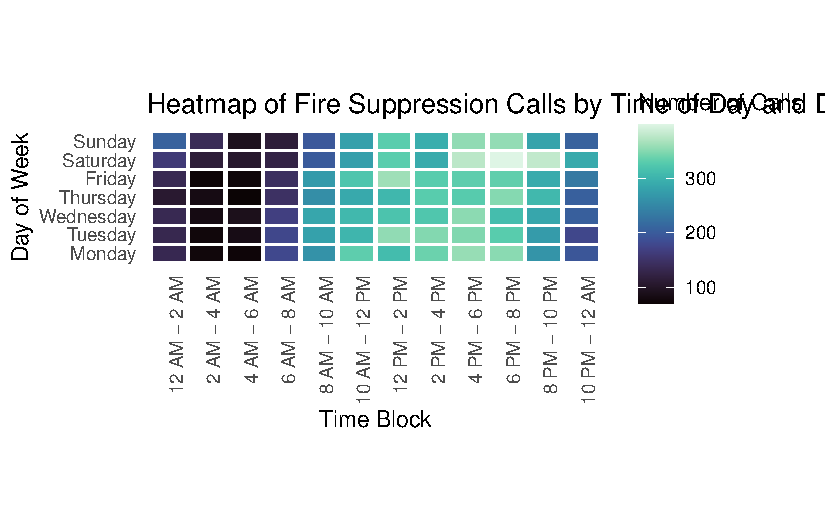
\includegraphics{Report_files/figure-pdf/exploratory_2-1.pdf}

}

\caption{Heatmap by Day of Week and Time of Day}

}

\end{minipage}%

\end{figure}

Now, let us look directly at how the number of calls vary across the
time of day, grouped by the day of week and month respectively.

\hypertarget{heat-map-of}{%
\paragraph{Heat map of}\label{heat-map-of}}

\begin{Shaded}
\begin{Highlighting}[]
\CommentTok{\# Aggregate calls by day\_of\_week and block}
\NormalTok{aggregated\_data }\OtherTok{\textless{}{-}}\NormalTok{ data }\SpecialCharTok{\%\textgreater{}\%}
  \FunctionTok{group\_by}\NormalTok{(Day.of.week, block) }\SpecialCharTok{\%\textgreater{}\%}
  \FunctionTok{summarise}\NormalTok{(}\AttributeTok{call\_count =} \FunctionTok{n}\NormalTok{()) }\SpecialCharTok{\%\textgreater{}\%}
  \FunctionTok{ungroup}\NormalTok{()}

\CommentTok{\# Ensure the day\_of\_week is ordered from Monday to Sunday}
\NormalTok{aggregated\_data}\SpecialCharTok{$}\NormalTok{day\_of\_week }\OtherTok{\textless{}{-}} \FunctionTok{factor}\NormalTok{(aggregated\_data}\SpecialCharTok{$}\NormalTok{Day.of.week, }
                                     \AttributeTok{levels =} \FunctionTok{c}\NormalTok{(}\StringTok{"Monday"}\NormalTok{, }\StringTok{"Tuesday"}\NormalTok{, }\StringTok{"Wednesday"}\NormalTok{, }\StringTok{"Thursday"}\NormalTok{, }
                                                \StringTok{"Friday"}\NormalTok{, }\StringTok{"Saturday"}\NormalTok{, }\StringTok{"Sunday"}\NormalTok{))}

\CommentTok{\# Create the heatmap}
\NormalTok{heatmap\_plot }\OtherTok{\textless{}{-}} \FunctionTok{ggplot}\NormalTok{(aggregated\_data, }\FunctionTok{aes}\NormalTok{(}\AttributeTok{x =}\NormalTok{ block, }\AttributeTok{y =}\NormalTok{ day\_of\_week, }\AttributeTok{fill =}\NormalTok{ call\_count)) }\SpecialCharTok{+}
  \FunctionTok{geom\_tile}\NormalTok{(}\AttributeTok{color =} \StringTok{"white"}\NormalTok{) }\SpecialCharTok{+}
  \FunctionTok{scale\_fill\_viridis}\NormalTok{(}\AttributeTok{name =} \StringTok{"Number of Calls"}\NormalTok{, }\AttributeTok{option =} \StringTok{"G"}\NormalTok{) }\SpecialCharTok{+}
  \FunctionTok{labs}\NormalTok{(}\AttributeTok{title =} \StringTok{"Heatmap of Fire Suppression Calls by Time of Day and Day of Week"}\NormalTok{,}
       \AttributeTok{x =} \StringTok{"Time Block"}\NormalTok{,}
       \AttributeTok{y =} \StringTok{"Day of Week"}\NormalTok{) }\SpecialCharTok{+}
  \FunctionTok{theme\_minimal}\NormalTok{() }\SpecialCharTok{+}
  \FunctionTok{theme}\NormalTok{(}\AttributeTok{axis.text.x =} \FunctionTok{element\_text}\NormalTok{(}\AttributeTok{angle =} \DecValTok{45}\NormalTok{, }\AttributeTok{hjust =} \DecValTok{1}\NormalTok{),}
        \AttributeTok{panel.grid =} \FunctionTok{element\_blank}\NormalTok{())}

\CommentTok{\# Display the heatmap}
\FunctionTok{print}\NormalTok{(heatmap\_plot)}
\end{Highlighting}
\end{Shaded}

\begin{figure}[H]

{\centering 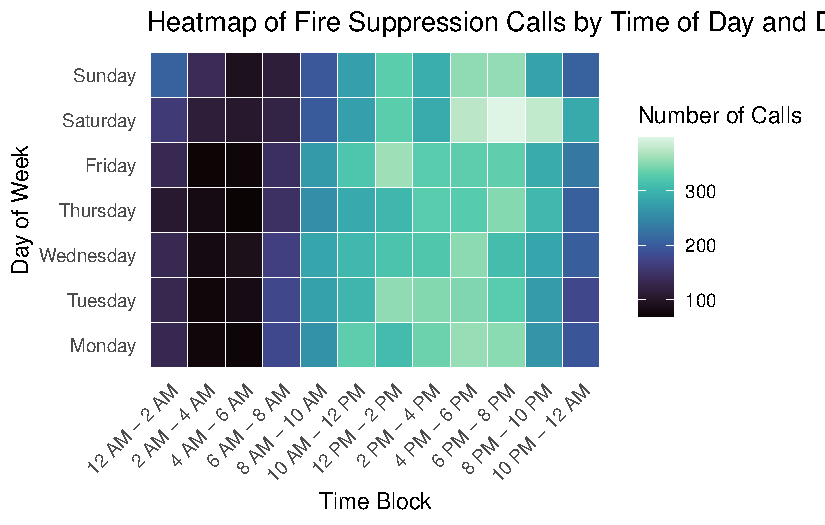
\includegraphics{Report_files/figure-pdf/unnamed-chunk-5-1.pdf}

}

\end{figure}

\hypertarget{identifying-holidays-and-weekends}{%
\subsubsection{Identifying Holidays and
Weekends}\label{identifying-holidays-and-weekends}}

\hypertarget{holidays}{%
\paragraph{Holidays}\label{holidays}}

\begin{Shaded}
\begin{Highlighting}[]
\CommentTok{\# List of US holidays}
\NormalTok{us\_holidays }\OtherTok{\textless{}{-}} \FunctionTok{as.Date}\NormalTok{(}\FunctionTok{holidayNYSE}\NormalTok{(}\FunctionTok{unique}\NormalTok{(}\FunctionTok{year}\NormalTok{(data}\SpecialCharTok{$}\NormalTok{dispatched))))}

\CommentTok{\# Add holiday indicator}
\NormalTok{data }\OtherTok{\textless{}{-}}\NormalTok{ data }\SpecialCharTok{\%\textgreater{}\%}
  \FunctionTok{mutate}\NormalTok{(}\AttributeTok{is\_holiday =} \FunctionTok{if\_else}\NormalTok{(dispatched }\SpecialCharTok{\%in\%}\NormalTok{ us\_holidays, }\DecValTok{1}\NormalTok{, }\DecValTok{0}\NormalTok{))}

\CommentTok{\# Total number of days in the dataset}
\NormalTok{total\_days }\OtherTok{\textless{}{-}}\NormalTok{ data }\SpecialCharTok{\%\textgreater{}\%}
  \FunctionTok{summarise}\NormalTok{(}\AttributeTok{days =} \FunctionTok{n\_distinct}\NormalTok{(dispatched)) }\SpecialCharTok{\%\textgreater{}\%}
  \FunctionTok{pull}\NormalTok{(days)}

\CommentTok{\# Number of holiday days}
\NormalTok{num\_holiday\_days }\OtherTok{\textless{}{-}}\NormalTok{ data }\SpecialCharTok{\%\textgreater{}\%}
  \FunctionTok{filter}\NormalTok{(is\_holiday }\SpecialCharTok{==} \DecValTok{1}\NormalTok{) }\SpecialCharTok{\%\textgreater{}\%}
  \FunctionTok{summarise}\NormalTok{(}\AttributeTok{days =} \FunctionTok{n\_distinct}\NormalTok{(dispatched)) }\SpecialCharTok{\%\textgreater{}\%}
  \FunctionTok{pull}\NormalTok{(days)}

\CommentTok{\# Number of non{-}holiday days}
\NormalTok{num\_non\_holiday\_days }\OtherTok{\textless{}{-}}\NormalTok{ total\_days }\SpecialCharTok{{-}}\NormalTok{ num\_holiday\_days}

\FunctionTok{cat}\NormalTok{(}\StringTok{"Total Days:"}\NormalTok{, total\_days, }\StringTok{"}\SpecialCharTok{\textbackslash{}n}\StringTok{"}\NormalTok{)}
\end{Highlighting}
\end{Shaded}

\begin{verbatim}
Total Days: 3313 
\end{verbatim}

\begin{Shaded}
\begin{Highlighting}[]
\FunctionTok{cat}\NormalTok{(}\StringTok{"Holiday Days:"}\NormalTok{, num\_holiday\_days, }\StringTok{"}\SpecialCharTok{\textbackslash{}n}\StringTok{"}\NormalTok{)}
\end{Highlighting}
\end{Shaded}

\begin{verbatim}
Holiday Days: 83 
\end{verbatim}

\begin{Shaded}
\begin{Highlighting}[]
\FunctionTok{cat}\NormalTok{(}\StringTok{"Non{-}Holiday Days:"}\NormalTok{, num\_non\_holiday\_days, }\StringTok{"}\SpecialCharTok{\textbackslash{}n}\StringTok{"}\NormalTok{)}
\end{Highlighting}
\end{Shaded}

\begin{verbatim}
Non-Holiday Days: 3230 
\end{verbatim}

\begin{Shaded}
\begin{Highlighting}[]
\CommentTok{\# Total calls on holidays}
\NormalTok{total\_calls\_holiday }\OtherTok{\textless{}{-}}\NormalTok{ data }\SpecialCharTok{\%\textgreater{}\%}
  \FunctionTok{filter}\NormalTok{(is\_holiday }\SpecialCharTok{==} \DecValTok{1}\NormalTok{) }\SpecialCharTok{\%\textgreater{}\%}
  \FunctionTok{summarise}\NormalTok{(}\AttributeTok{total\_calls =} \FunctionTok{n}\NormalTok{()) }\SpecialCharTok{\%\textgreater{}\%}
  \FunctionTok{pull}\NormalTok{(total\_calls)}

\CommentTok{\# Total calls on non{-}holidays}
\NormalTok{total\_calls\_non\_holiday }\OtherTok{\textless{}{-}}\NormalTok{ data }\SpecialCharTok{\%\textgreater{}\%}
  \FunctionTok{filter}\NormalTok{(is\_holiday }\SpecialCharTok{==} \DecValTok{0}\NormalTok{) }\SpecialCharTok{\%\textgreater{}\%}
  \FunctionTok{summarise}\NormalTok{(}\AttributeTok{total\_calls =} \FunctionTok{n}\NormalTok{()) }\SpecialCharTok{\%\textgreater{}\%}
  \FunctionTok{pull}\NormalTok{(total\_calls)}

\CommentTok{\# Average calls per holiday}
\NormalTok{avg\_calls\_per\_holiday }\OtherTok{\textless{}{-}}\NormalTok{ total\_calls\_holiday }\SpecialCharTok{/}\NormalTok{ num\_holiday\_days}

\CommentTok{\# Average calls per non{-}holiday}
\NormalTok{avg\_calls\_per\_non\_holiday }\OtherTok{\textless{}{-}}\NormalTok{ total\_calls\_non\_holiday }\SpecialCharTok{/}\NormalTok{ num\_non\_holiday\_days}

\FunctionTok{cat}\NormalTok{(}\StringTok{"Average Calls per Holiday:"}\NormalTok{, avg\_calls\_per\_holiday, }\StringTok{"}\SpecialCharTok{\textbackslash{}n}\StringTok{"}\NormalTok{)}
\end{Highlighting}
\end{Shaded}

\begin{verbatim}
Average Calls per Holiday: 6.421687 
\end{verbatim}

\begin{Shaded}
\begin{Highlighting}[]
\FunctionTok{cat}\NormalTok{(}\StringTok{"Average Calls per Non{-}Holiday:"}\NormalTok{, avg\_calls\_per\_non\_holiday, }\StringTok{"}\SpecialCharTok{\textbackslash{}n}\StringTok{"}\NormalTok{)}
\end{Highlighting}
\end{Shaded}

\begin{verbatim}
Average Calls per Non-Holiday: 6.081424 
\end{verbatim}

\begin{Shaded}
\begin{Highlighting}[]
\CommentTok{\# Create a data frame for plotting}
\NormalTok{holiday\_avg\_calls }\OtherTok{\textless{}{-}} \FunctionTok{tibble}\NormalTok{(}
  \AttributeTok{Day\_Type =} \FunctionTok{c}\NormalTok{(}\StringTok{"Holiday"}\NormalTok{, }\StringTok{"Non{-}Holiday"}\NormalTok{),}
  \AttributeTok{Average\_Calls =} \FunctionTok{c}\NormalTok{(avg\_calls\_per\_holiday, avg\_calls\_per\_non\_holiday)}
\NormalTok{)}

\CommentTok{\# Plot calls by holiday indicator}
\NormalTok{data }\SpecialCharTok{\%\textgreater{}\%}
  \FunctionTok{count}\NormalTok{(is\_holiday) }\SpecialCharTok{\%\textgreater{}\%}
  \FunctionTok{ggplot}\NormalTok{(}\FunctionTok{aes}\NormalTok{(}\AttributeTok{x =} \FunctionTok{factor}\NormalTok{(is\_holiday, }\AttributeTok{labels =} \FunctionTok{c}\NormalTok{(}\StringTok{"Non{-}Holiday"}\NormalTok{, }\StringTok{"Holiday"}\NormalTok{)), }\AttributeTok{y =}\NormalTok{ n)) }\SpecialCharTok{+}
  \FunctionTok{geom\_bar}\NormalTok{(}\AttributeTok{stat =} \StringTok{"identity"}\NormalTok{, }\AttributeTok{fill =} \StringTok{"coral"}\NormalTok{) }\SpecialCharTok{+}
  \FunctionTok{labs}\NormalTok{(}\AttributeTok{title =} \StringTok{"Number of Calls Per Day on Holidays vs Non{-}Holidays"}\NormalTok{, }\AttributeTok{x =} \StringTok{"Day Type"}\NormalTok{, }\AttributeTok{y =} \StringTok{"Number of Calls"}\NormalTok{) }\SpecialCharTok{+} \FunctionTok{theme\_minimal}\NormalTok{()}
\end{Highlighting}
\end{Shaded}

\begin{figure}[H]

{\centering 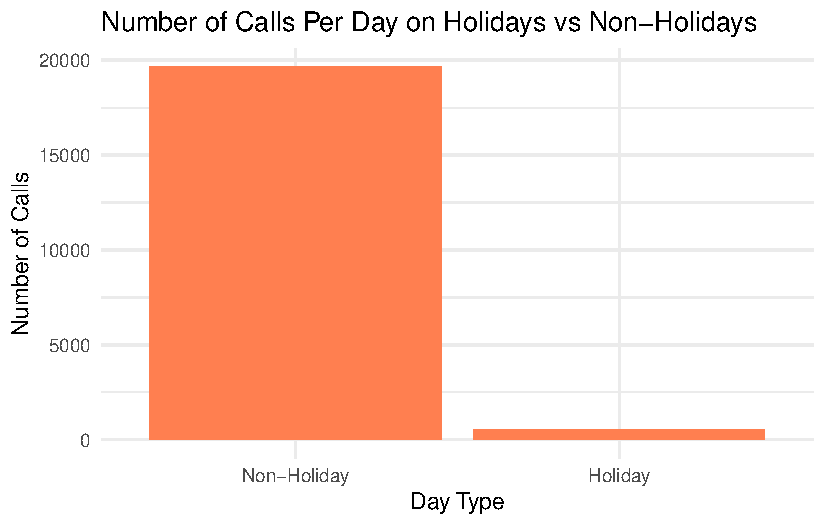
\includegraphics{Report_files/figure-pdf/unnamed-chunk-6-1.pdf}

}

\end{figure}

\begin{Shaded}
\begin{Highlighting}[]
\CommentTok{\# Plot}
\NormalTok{holiday\_avg\_calls }\SpecialCharTok{\%\textgreater{}\%}
  \FunctionTok{ggplot}\NormalTok{(}\FunctionTok{aes}\NormalTok{(}\AttributeTok{x =}\NormalTok{ Day\_Type, }\AttributeTok{y =}\NormalTok{ Average\_Calls, }\AttributeTok{fill =}\NormalTok{ Day\_Type)) }\SpecialCharTok{+}
  \FunctionTok{geom\_bar}\NormalTok{(}\AttributeTok{stat =} \StringTok{"identity"}\NormalTok{) }\SpecialCharTok{+}
  \FunctionTok{labs}\NormalTok{(}\AttributeTok{title =} \StringTok{"Average Calls per Day: Holidays vs Non{-}Holidays"}\NormalTok{, }\AttributeTok{x =} \StringTok{"Day Type"}\NormalTok{, }\AttributeTok{y =} \StringTok{"Average Calls per Day"}\NormalTok{) }\SpecialCharTok{+}
  \FunctionTok{theme\_minimal}\NormalTok{()}
\end{Highlighting}
\end{Shaded}

\begin{figure}[H]

{\centering 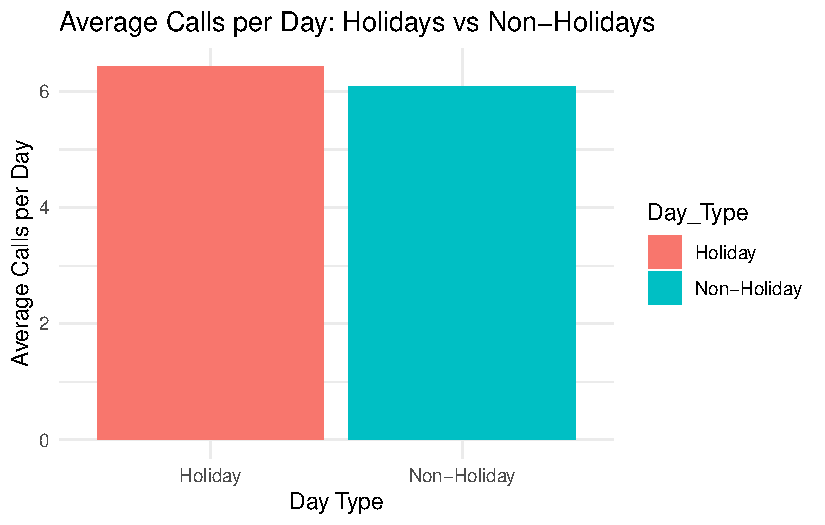
\includegraphics{Report_files/figure-pdf/unnamed-chunk-6-2.pdf}

}

\end{figure}

\begin{Shaded}
\begin{Highlighting}[]
\CommentTok{\# Daily call counts}
\NormalTok{daily\_calls }\OtherTok{\textless{}{-}}\NormalTok{ data }\SpecialCharTok{\%\textgreater{}\%}
  \FunctionTok{group\_by}\NormalTok{(dispatched, is\_holiday) }\SpecialCharTok{\%\textgreater{}\%}
  \FunctionTok{summarise}\NormalTok{(}\AttributeTok{calls =} \FunctionTok{n}\NormalTok{()) }\SpecialCharTok{\%\textgreater{}\%}
  \FunctionTok{ungroup}\NormalTok{()}

\CommentTok{\# Split into holiday and non{-}holiday datasets}
\NormalTok{calls\_holiday }\OtherTok{\textless{}{-}}\NormalTok{ daily\_calls }\SpecialCharTok{\%\textgreater{}\%}
  \FunctionTok{filter}\NormalTok{(is\_holiday }\SpecialCharTok{==} \DecValTok{1}\NormalTok{) }\SpecialCharTok{\%\textgreater{}\%}
  \FunctionTok{pull}\NormalTok{(calls)}

\NormalTok{calls\_non\_holiday }\OtherTok{\textless{}{-}}\NormalTok{ daily\_calls }\SpecialCharTok{\%\textgreater{}\%}
  \FunctionTok{filter}\NormalTok{(is\_holiday }\SpecialCharTok{==} \DecValTok{0}\NormalTok{) }\SpecialCharTok{\%\textgreater{}\%}
  \FunctionTok{pull}\NormalTok{(calls)}

\CommentTok{\# Shapiro{-}Wilk test for normality}
\FunctionTok{shapiro.test}\NormalTok{(calls\_holiday)}
\end{Highlighting}
\end{Shaded}

\begin{verbatim}

    Shapiro-Wilk normality test

data:  calls_holiday
W = 0.9707, p-value = 0.05473
\end{verbatim}

\begin{Shaded}
\begin{Highlighting}[]
\FunctionTok{shapiro.test}\NormalTok{(calls\_non\_holiday)}
\end{Highlighting}
\end{Shaded}

\begin{verbatim}

    Shapiro-Wilk normality test

data:  calls_non_holiday
W = 0.97131, p-value < 2.2e-16
\end{verbatim}

\hypertarget{weekends}{%
\paragraph{Weekends}\label{weekends}}

\begin{Shaded}
\begin{Highlighting}[]
\CommentTok{\# Add weekend indicator}
\NormalTok{data }\OtherTok{\textless{}{-}}\NormalTok{ data }\SpecialCharTok{\%\textgreater{}\%}
  \FunctionTok{mutate}\NormalTok{(}\AttributeTok{is\_weekend =} \FunctionTok{if\_else}\NormalTok{(Day.of.week }\SpecialCharTok{\%in\%} \FunctionTok{c}\NormalTok{(}\StringTok{"Friday"}\NormalTok{, }\StringTok{"Saturday"}\NormalTok{), }\DecValTok{1}\NormalTok{, }\DecValTok{0}\NormalTok{))}

\CommentTok{\# Number of weekend days}
\NormalTok{num\_weekend\_days }\OtherTok{\textless{}{-}}\NormalTok{ data }\SpecialCharTok{\%\textgreater{}\%}
  \FunctionTok{filter}\NormalTok{(is\_weekend }\SpecialCharTok{==} \DecValTok{1}\NormalTok{) }\SpecialCharTok{\%\textgreater{}\%}
  \FunctionTok{summarise}\NormalTok{(}\AttributeTok{days =} \FunctionTok{n\_distinct}\NormalTok{(dispatched)) }\SpecialCharTok{\%\textgreater{}\%}
  \FunctionTok{pull}\NormalTok{(days)}

\CommentTok{\# Number of weekday days}
\NormalTok{num\_weekday\_days }\OtherTok{\textless{}{-}}\NormalTok{ total\_days }\SpecialCharTok{{-}}\NormalTok{ num\_weekend\_days}

\FunctionTok{cat}\NormalTok{(}\StringTok{"Weekend Days:"}\NormalTok{, num\_weekend\_days, }\StringTok{"}\SpecialCharTok{\textbackslash{}n}\StringTok{"}\NormalTok{)}
\end{Highlighting}
\end{Shaded}

\begin{verbatim}
Weekend Days: 943 
\end{verbatim}

\begin{Shaded}
\begin{Highlighting}[]
\FunctionTok{cat}\NormalTok{(}\StringTok{"Weekday Days:"}\NormalTok{, num\_weekday\_days, }\StringTok{"}\SpecialCharTok{\textbackslash{}n}\StringTok{"}\NormalTok{)}
\end{Highlighting}
\end{Shaded}

\begin{verbatim}
Weekday Days: 2370 
\end{verbatim}

\begin{Shaded}
\begin{Highlighting}[]
\CommentTok{\# Total calls on weekends}
\NormalTok{total\_calls\_weekend }\OtherTok{\textless{}{-}}\NormalTok{ data }\SpecialCharTok{\%\textgreater{}\%}
  \FunctionTok{filter}\NormalTok{(is\_weekend }\SpecialCharTok{==} \DecValTok{1}\NormalTok{) }\SpecialCharTok{\%\textgreater{}\%}
  \FunctionTok{summarise}\NormalTok{(}\AttributeTok{total\_calls =} \FunctionTok{n}\NormalTok{()) }\SpecialCharTok{\%\textgreater{}\%}
  \FunctionTok{pull}\NormalTok{(total\_calls)}

\CommentTok{\# Total calls on weekdays}
\NormalTok{total\_calls\_weekday }\OtherTok{\textless{}{-}}\NormalTok{ data }\SpecialCharTok{\%\textgreater{}\%}
  \FunctionTok{filter}\NormalTok{(is\_weekend }\SpecialCharTok{==} \DecValTok{0}\NormalTok{) }\SpecialCharTok{\%\textgreater{}\%}
  \FunctionTok{summarise}\NormalTok{(}\AttributeTok{total\_calls =} \FunctionTok{n}\NormalTok{()) }\SpecialCharTok{\%\textgreater{}\%}
  \FunctionTok{pull}\NormalTok{(total\_calls)}

\CommentTok{\# Average calls per weekend day}
\NormalTok{avg\_calls\_per\_weekend }\OtherTok{\textless{}{-}}\NormalTok{ total\_calls\_weekend }\SpecialCharTok{/}\NormalTok{ num\_weekend\_days}

\CommentTok{\# Average calls per weekday}
\NormalTok{avg\_calls\_per\_weekday }\OtherTok{\textless{}{-}}\NormalTok{ total\_calls\_weekday }\SpecialCharTok{/}\NormalTok{ num\_weekday\_days}

\FunctionTok{cat}\NormalTok{(}\StringTok{"Average Calls per Weekend Day:"}\NormalTok{, avg\_calls\_per\_weekend, }\StringTok{"}\SpecialCharTok{\textbackslash{}n}\StringTok{"}\NormalTok{)}
\end{Highlighting}
\end{Shaded}

\begin{verbatim}
Average Calls per Weekend Day: 6.296925 
\end{verbatim}

\begin{Shaded}
\begin{Highlighting}[]
\FunctionTok{cat}\NormalTok{(}\StringTok{"Average Calls per Weekday:"}\NormalTok{, avg\_calls\_per\_weekday, }\StringTok{"}\SpecialCharTok{\textbackslash{}n}\StringTok{"}\NormalTok{)}
\end{Highlighting}
\end{Shaded}

\begin{verbatim}
Average Calls per Weekday: 6.007595 
\end{verbatim}

\begin{Shaded}
\begin{Highlighting}[]
\CommentTok{\# Plot calls by weekend indicator}
\NormalTok{data }\SpecialCharTok{\%\textgreater{}\%}
  \FunctionTok{count}\NormalTok{(is\_weekend) }\SpecialCharTok{\%\textgreater{}\%}
  \FunctionTok{ggplot}\NormalTok{(}\FunctionTok{aes}\NormalTok{(}\AttributeTok{x =} \FunctionTok{factor}\NormalTok{(is\_weekend, }\AttributeTok{labels =} \FunctionTok{c}\NormalTok{(}\StringTok{"Weekday"}\NormalTok{, }\StringTok{"Weekend"}\NormalTok{)), }\AttributeTok{y =}\NormalTok{ n)) }\SpecialCharTok{+}
  \FunctionTok{geom\_bar}\NormalTok{(}\AttributeTok{stat =} \StringTok{"identity"}\NormalTok{, }\AttributeTok{fill =} \StringTok{"steelblue"}\NormalTok{) }\SpecialCharTok{+}
  \FunctionTok{labs}\NormalTok{(}\AttributeTok{title =} \StringTok{"Number of Calls Per Day on Weekends vs Weekdays"}\NormalTok{, }\AttributeTok{x =} \StringTok{"Day Type"}\NormalTok{, }\AttributeTok{y =} \StringTok{"Number of Calls"}\NormalTok{) }\SpecialCharTok{+} \FunctionTok{theme\_minimal}\NormalTok{()}
\end{Highlighting}
\end{Shaded}

\begin{figure}[H]

{\centering 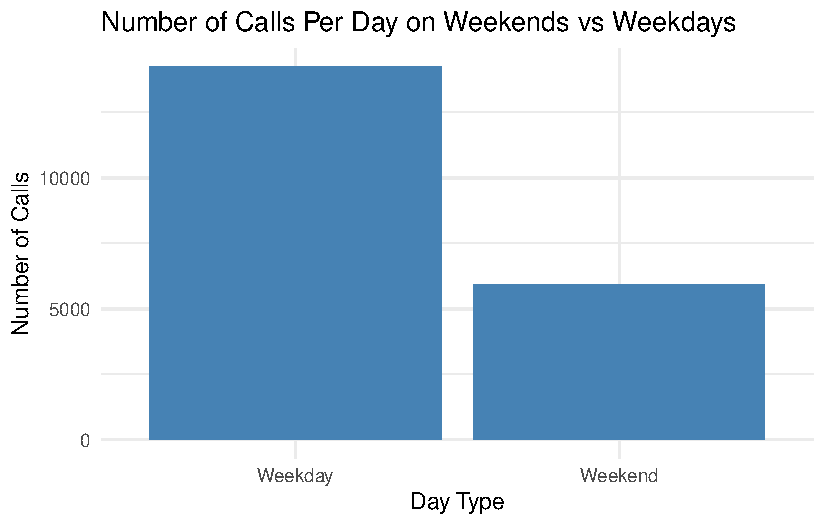
\includegraphics{Report_files/figure-pdf/unnamed-chunk-7-1.pdf}

}

\end{figure}

\begin{Shaded}
\begin{Highlighting}[]
\CommentTok{\# Create a data frame for plotting}
\NormalTok{weekend\_avg\_calls }\OtherTok{\textless{}{-}} \FunctionTok{tibble}\NormalTok{(}
  \AttributeTok{Day\_Type =} \FunctionTok{c}\NormalTok{(}\StringTok{"Weekend"}\NormalTok{, }\StringTok{"Weekday"}\NormalTok{),}
  \AttributeTok{Average\_Calls =} \FunctionTok{c}\NormalTok{(avg\_calls\_per\_weekend, avg\_calls\_per\_weekday)}
\NormalTok{)}

\CommentTok{\# Plot}
\NormalTok{weekend\_avg\_calls }\SpecialCharTok{\%\textgreater{}\%}
  \FunctionTok{ggplot}\NormalTok{(}\FunctionTok{aes}\NormalTok{(}\AttributeTok{x =}\NormalTok{ Day\_Type, }\AttributeTok{y =}\NormalTok{ Average\_Calls, }\AttributeTok{fill =}\NormalTok{ Day\_Type)) }\SpecialCharTok{+}
  \FunctionTok{geom\_bar}\NormalTok{(}\AttributeTok{stat =} \StringTok{"identity"}\NormalTok{) }\SpecialCharTok{+}
  \FunctionTok{labs}\NormalTok{(}\AttributeTok{title =} \StringTok{"Average Calls per Day: Weekends vs Weekdays"}\NormalTok{, }\AttributeTok{x =} \StringTok{"Day Type"}\NormalTok{, }\AttributeTok{y =} \StringTok{"Average Calls per Day"}\NormalTok{) }\SpecialCharTok{+}
  \FunctionTok{theme\_minimal}\NormalTok{()}
\end{Highlighting}
\end{Shaded}

\begin{figure}[H]

{\centering 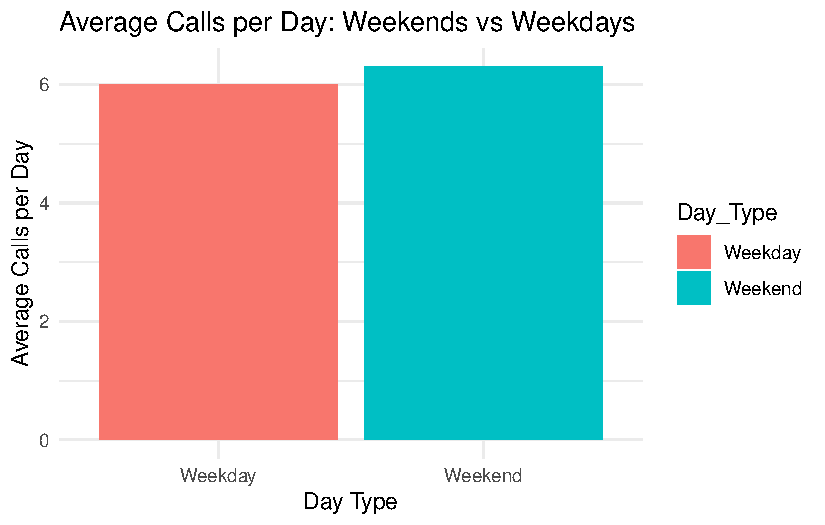
\includegraphics{Report_files/figure-pdf/unnamed-chunk-7-2.pdf}

}

\end{figure}

\hypertarget{modeling}{%
\subsection{Modeling}\label{modeling}}

\begin{Shaded}
\begin{Highlighting}[]
\NormalTok{day.unique }\OtherTok{=} \FunctionTok{unique}\NormalTok{(data}\SpecialCharTok{$}\NormalTok{dispatched)}
\NormalTok{block.unique }\OtherTok{=} \FunctionTok{unique}\NormalTok{(data}\SpecialCharTok{$}\NormalTok{hour)}
\NormalTok{clean.df }\OtherTok{=} \FunctionTok{expand\_grid}\NormalTok{(day.unique, block.unique)}
\NormalTok{clean.df }\OtherTok{=}\NormalTok{ clean.df }\SpecialCharTok{\%\textgreater{}\%} 
  \FunctionTok{left\_join}\NormalTok{(}
\NormalTok{    data }\SpecialCharTok{\%\textgreater{}\%} \FunctionTok{group\_by}\NormalTok{(dispatched, hour) }\SpecialCharTok{\%\textgreater{}\%} \FunctionTok{summarize}\NormalTok{(}\AttributeTok{call =} \FunctionTok{n}\NormalTok{()),}
    \AttributeTok{by =} \FunctionTok{c}\NormalTok{(}\StringTok{"day.unique"} \OtherTok{=} \StringTok{"dispatched"}\NormalTok{, }\StringTok{"block.unique"} \OtherTok{=} \StringTok{"hour"}\NormalTok{)}
\NormalTok{  )}
\NormalTok{clean.df }\OtherTok{=}\NormalTok{ clean.df }\SpecialCharTok{\%\textgreater{}\%} \FunctionTok{mutate}\NormalTok{(}\AttributeTok{count =} \FunctionTok{case\_when}\NormalTok{(}\FunctionTok{is.na}\NormalTok{(call) }\SpecialCharTok{\textasciitilde{}} \DecValTok{0}\NormalTok{,}
                                      \AttributeTok{.default =}\NormalTok{ call))}
\end{Highlighting}
\end{Shaded}

\begin{Shaded}
\begin{Highlighting}[]
\FunctionTok{library}\NormalTok{(mgcv)}
\NormalTok{model }\OtherTok{=} \FunctionTok{gam}\NormalTok{(count }\SpecialCharTok{\textasciitilde{}} \FunctionTok{s}\NormalTok{(block.unique), }\AttributeTok{data =}\NormalTok{ clean.df)}
\end{Highlighting}
\end{Shaded}

\begin{Shaded}
\begin{Highlighting}[]
\FunctionTok{set.seed}\NormalTok{(}\DecValTok{123}\NormalTok{)}
\NormalTok{split }\OtherTok{\textless{}{-}} \FunctionTok{initial\_split}\NormalTok{(clean.df, }\AttributeTok{prop =} \FloatTok{0.8}\NormalTok{)}
\NormalTok{train\_data }\OtherTok{\textless{}{-}} \FunctionTok{training}\NormalTok{(split)}
\NormalTok{test\_data }\OtherTok{\textless{}{-}} \FunctionTok{testing}\NormalTok{(split)}
\end{Highlighting}
\end{Shaded}

\begin{Shaded}
\begin{Highlighting}[]
\NormalTok{model }\OtherTok{=} \FunctionTok{gam}\NormalTok{(count }\SpecialCharTok{\textasciitilde{}} \FunctionTok{s}\NormalTok{(block.unique), }\AttributeTok{data =}\NormalTok{ train\_data, }\AttributeTok{family =}\NormalTok{ poisson)}
\end{Highlighting}
\end{Shaded}

\begin{Shaded}
\begin{Highlighting}[]
\NormalTok{predict }\OtherTok{=} \FunctionTok{predict.gam}\NormalTok{(model, test\_data, }\AttributeTok{type =} \StringTok{"response"}\NormalTok{, }\AttributeTok{se.fit =} \ConstantTok{TRUE}\NormalTok{)}
\end{Highlighting}
\end{Shaded}

\begin{Shaded}
\begin{Highlighting}[]
\NormalTok{fitted\_values }\OtherTok{=}\NormalTok{ predict}\SpecialCharTok{$}\NormalTok{fit}
\NormalTok{se\_values }\OtherTok{=}\NormalTok{ predict}\SpecialCharTok{$}\NormalTok{se.fit}

\NormalTok{lower\_bound }\OtherTok{=}\NormalTok{ fitted\_values }\SpecialCharTok{{-}} \FloatTok{1.96} \SpecialCharTok{*}\NormalTok{ se\_values}
\NormalTok{upper\_bound }\OtherTok{=}\NormalTok{ fitted\_values }\SpecialCharTok{+} \FloatTok{1.96} \SpecialCharTok{*}\NormalTok{ se\_values}

\NormalTok{result }\OtherTok{=} \FunctionTok{data.frame}\NormalTok{(}
  \AttributeTok{day\_unique =}\NormalTok{ test\_data}\SpecialCharTok{$}\NormalTok{day.unique,}
  \AttributeTok{block\_unique =}\NormalTok{ test\_data}\SpecialCharTok{$}\NormalTok{block.unique,}
  \AttributeTok{fitted\_values =}\NormalTok{ fitted\_values,}
  \AttributeTok{lower\_bound =}\NormalTok{ lower\_bound,}
  \AttributeTok{upper\_bound =}\NormalTok{ upper\_bound,}
  \AttributeTok{count =}\NormalTok{ test\_data}\SpecialCharTok{$}\NormalTok{count}
\NormalTok{)}

\NormalTok{p }\OtherTok{\textless{}{-}} \FunctionTok{ggplot}\NormalTok{(}\AttributeTok{data =}\NormalTok{ result, }\FunctionTok{aes}\NormalTok{(}\AttributeTok{x =}\NormalTok{ block\_unique, }\AttributeTok{y =}\NormalTok{ fitted\_values)) }\SpecialCharTok{+}
  \FunctionTok{geom\_ribbon}\NormalTok{(}\FunctionTok{aes}\NormalTok{(}\AttributeTok{ymin =}\NormalTok{ lower\_bound, }\AttributeTok{ymax =}\NormalTok{ upper\_bound), }
              \AttributeTok{fill =} \StringTok{"steelblue"}\NormalTok{, }
              \AttributeTok{alpha =} \FloatTok{0.3}\NormalTok{) }\SpecialCharTok{+}
  \FunctionTok{geom\_line}\NormalTok{(}\AttributeTok{color =} \StringTok{"steelblue"}\NormalTok{, }\AttributeTok{size =} \DecValTok{1}\NormalTok{) }\SpecialCharTok{+} 
  \FunctionTok{labs}\NormalTok{(}
    \AttributeTok{title =} \StringTok{"Expected Number of Calls by Time of Day"}\NormalTok{,}
    \AttributeTok{subtitle =} \StringTok{"Confidence Intervals Representing 95\% Prediction Bounds"}\NormalTok{,}
    \AttributeTok{x =} \StringTok{"Time of Day"}\NormalTok{,}
    \AttributeTok{y =} \StringTok{"Expected Number of Calls"}
\NormalTok{  ) }\SpecialCharTok{+}
  \FunctionTok{scale\_x\_continuous}\NormalTok{(}
    \AttributeTok{breaks =} \DecValTok{0}\SpecialCharTok{:}\DecValTok{23}\NormalTok{, }
    \AttributeTok{labels =} \FunctionTok{c}\NormalTok{(}\StringTok{"12:00 AM"}\NormalTok{, }\StringTok{"1:00 AM"}\NormalTok{, }\StringTok{"2:00 AM"}\NormalTok{, }\StringTok{"3:00 AM"}\NormalTok{, }\StringTok{"4:00 AM"}\NormalTok{, }
               \StringTok{"5:00 AM"}\NormalTok{, }\StringTok{"6:00 AM"}\NormalTok{, }\StringTok{"7:00 AM"}\NormalTok{, }\StringTok{"8:00 AM"}\NormalTok{, }\StringTok{"9:00 AM"}\NormalTok{, }
               \StringTok{"10:00 AM"}\NormalTok{, }\StringTok{"11:00 AM"}\NormalTok{, }\StringTok{"12:00 PM"}\NormalTok{, }\StringTok{"1:00 PM"}\NormalTok{, }\StringTok{"2:00 PM"}\NormalTok{, }
               \StringTok{"3:00 PM"}\NormalTok{, }\StringTok{"4:00 PM"}\NormalTok{, }\StringTok{"5:00 PM"}\NormalTok{, }\StringTok{"6:00 PM"}\NormalTok{, }\StringTok{"7:00 PM"}\NormalTok{, }
               \StringTok{"8:00 PM"}\NormalTok{, }\StringTok{"9:00 PM"}\NormalTok{, }\StringTok{"10:00 PM"}\NormalTok{, }\StringTok{"11:00 PM"}\NormalTok{),}
    \AttributeTok{expand =} \FunctionTok{c}\NormalTok{(}\DecValTok{0}\NormalTok{, }\DecValTok{0}\NormalTok{)}
\NormalTok{  ) }\SpecialCharTok{+} 
  \FunctionTok{theme\_minimal}\NormalTok{(}\AttributeTok{base\_size =} \DecValTok{14}\NormalTok{) }\SpecialCharTok{+}
  \FunctionTok{theme}\NormalTok{(}
    \AttributeTok{axis.text.x =} \FunctionTok{element\_text}\NormalTok{(}\AttributeTok{angle =} \DecValTok{45}\NormalTok{, }\AttributeTok{hjust =} \DecValTok{1}\NormalTok{, }\AttributeTok{size =} \DecValTok{10}\NormalTok{, }\AttributeTok{color =} \StringTok{"gray30"}\NormalTok{),}
    \AttributeTok{plot.title =} \FunctionTok{element\_text}\NormalTok{(}\AttributeTok{face =} \StringTok{"bold"}\NormalTok{, }\AttributeTok{size =} \DecValTok{16}\NormalTok{, }\AttributeTok{hjust =} \FloatTok{0.5}\NormalTok{, }\AttributeTok{color =} \StringTok{"steelblue"}\NormalTok{),}
    \AttributeTok{plot.subtitle =} \FunctionTok{element\_text}\NormalTok{(}\AttributeTok{size =} \DecValTok{12}\NormalTok{, }\AttributeTok{hjust =} \FloatTok{0.5}\NormalTok{, }\AttributeTok{color =} \StringTok{"gray50"}\NormalTok{),}
    \AttributeTok{axis.title =} \FunctionTok{element\_text}\NormalTok{(}\AttributeTok{face =} \StringTok{"bold"}\NormalTok{, }\AttributeTok{size =} \DecValTok{12}\NormalTok{, }\AttributeTok{color =} \StringTok{"gray20"}\NormalTok{),}
    \AttributeTok{plot.caption =} \FunctionTok{element\_text}\NormalTok{(}\AttributeTok{size =} \DecValTok{10}\NormalTok{, }\AttributeTok{hjust =} \DecValTok{0}\NormalTok{, }\AttributeTok{color =} \StringTok{"gray50"}\NormalTok{),}
    \AttributeTok{panel.grid.major =} \FunctionTok{element\_line}\NormalTok{(}\AttributeTok{color =} \StringTok{"gray90"}\NormalTok{),}
    \AttributeTok{panel.grid.minor =} \FunctionTok{element\_blank}\NormalTok{(),}
    \AttributeTok{panel.background =} \FunctionTok{element\_rect}\NormalTok{(}\AttributeTok{fill =} \StringTok{"white"}\NormalTok{, }\AttributeTok{color =} \ConstantTok{NA}\NormalTok{)}
\NormalTok{  )}

\NormalTok{p}
\end{Highlighting}
\end{Shaded}

\begin{figure}[H]

{\centering 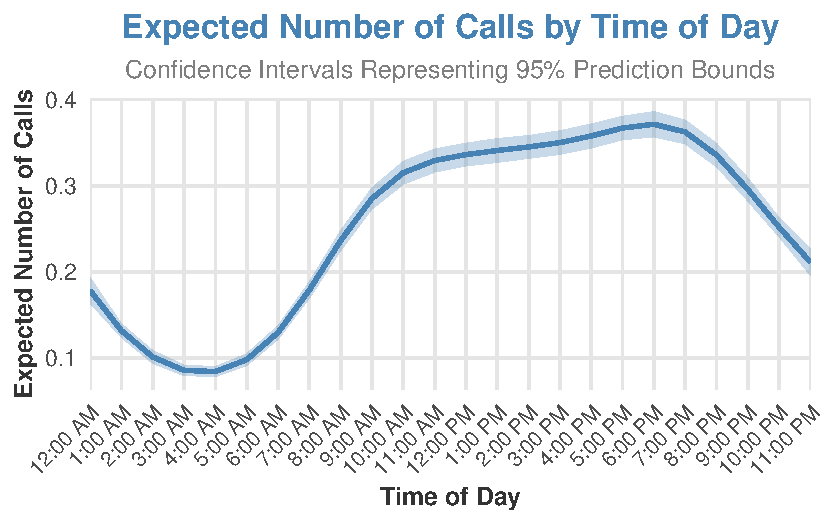
\includegraphics{Report_files/figure-pdf/unnamed-chunk-13-1.pdf}

}

\end{figure}



\end{document}
